\chapter{Literature Review}
% TODO \textbf{In this section you need to explain all the theory required to understand your dissertation (i.e.\ the following chapters)}

\noindent This chapter explores the foundational principles and advancements in document retrieval systems. It examines the traditional title and keyword-based search methods alongside the more sophisticated content-based approaches. A comparative analysis is provided, highlighting the strengths, limitations, and applications of these systems in addressing the evolving demands of users. By delving into the role of OCR, vector embeddings, and LLMs, this review sets the stage for evaluating how content-based systems redefine document retrieval processes in terms of accuracy, efficiency, and user satisfaction.

%! 2.1
\section{Document and Information Retrieval Systems}
\index{Document and Information Retrieval Systems|(}

\noindent In the modern era of digital transformation, organizations generate and store vast volumes of documents daily. This exponential growth in document storage has created an urgent need for efficient document retrieval systems (DRS) to access, manage, and utilize information effectively. A document retrieval system is a specialized application of information retrieval (IR) focused on locating relevant documents from a repository based on user queries. It plays a crucial role in knowledge management, decision-making, and enhancing productivity across various domains, including education, business, healthcare, and research.

Document retrieval is the problem of finding stored documents that contain useful information. According to Blaire et. al., (n.d.), There exist a set of documents on a range of topics, written by different authors, at different times, and at varying levels of depth, detail, clarity, and precision, and a set of individuals who, at different times and for different reasons, search for recorded information that may be contained in some of the documents in this set. In each instance in which an individual seeks information, he or she will find some documents of Ihe set useful and other documents not useful; the documents found useful are, we say. relevant; the others, not relevant. In order for a person to find all and only the relevant items in a collection of stored documents; one answer is automatic full-text retrieval, which on its surface is disarmingly simple: Store the full text of all documents in the collection on a computer so that every character of every word in every sentence of every document can be located by the machine. Then, when a person wants information from that stored collection, the computer is instructed to search for all documents containing certain specified words and word combinations, which the user has specified (MacDonald & Tonelleto, 2020).

\subsection{COIL: Revisit Exact Lexical Match in Information Retrieval with Contextualized Inverted List}

\noindent In the realm of information retrieval, traditional systems like BM25 have long relied on exact lexical matches, efficiently utilizing inverted list indexes to retrieve documents. However, these systems often struggle with vocabulary mismatches and fail to capture the semantic nuances of language. Conversely, recent neural information retrieval (IR) models emphasize soft semantic matching across all query-document terms, enhancing semantic understanding but at the cost of computational efficiency. Addressing this dichotomy, Gao, Dai, and Callan (2021) introduced the Contextualized Inverted List (COIL) architecture, which aims to integrate the efficiency of exact lexical matching with the semantic depth provided by deep language models.

COIL innovatively stores contextualized token representations within inverted lists, enabling the system to perform exact matches based on the contextual meaning of terms rather than solely on their surface forms. This approach allows COIL to leverage the rich semantic information captured by deep language models while maintaining the retrieval speed characteristic of traditional inverted index structures. By focusing on overlapping query-document tokens' contextualized representations, COIL effectively bridges the gap between lexical and semantic matching. Empirical evaluations demonstrate that COIL outperforms both classical lexical retrievers and state-of-the-art deep language model retrievers, achieving superior retrieval effectiveness with comparable or reduced latency. This performance underscores COIL's capability to deliver precise and contextually relevant results without compromising on efficiency.

The introduction of COIL represents a significant advancement in document and information retrieval systems. By harmonizing the strengths of exact lexical matching and semantic understanding, COIL addresses longstanding challenges such as vocabulary mismatch and semantic ambiguity. Its design offers a practical solution for developing retrieval systems that are both effective and efficient, making it a valuable reference for researchers and practitioners aiming to enhance retrieval performance in various applications.

\index{Document and Information Retrieval Systems!COIL: Revisit Exact Lexical Match in Information Retrieval with Contextualized Inverted List}

% TODO For sub-sub-section
% \subsubsection{Some Sub-sub-technique One}
% \blindtext

%! FOR PICTURE
% \begin{figure}[ht!] % supposedly places it here ...
%   \centering
%   
\includegraphics[width=0.6\linewidth]{test_image_goku}
%   \caption[This is the short caption for List of Figures]{A test figure.  This caption is huge, but in the list of figures only the smaller version in the square brackets will appear.\index{Goku il-king}}
%   \label{fig:test1}
% \end{figure}

% A test figure is shown in Figure~\ref{fig:test1}.

\index{Document and Information Retrieval Systems|)}

%! 2.2
\section{Embeddings in Document Retrieval}
\index{Embeddings in Document Retrieval|(}

\noindent In the realm of information retrieval, traditional methods have predominantly relied on keyword matching, which often falls short in capturing the nuanced meanings inherent in human language. This limitation has spurred the development of embedding techniques that represent words, sentences, and documents as vectors in high-dimensional space, effectively encoding semantic relationships. By transcending the constraints of exact keyword matches, embeddings facilitate a more profound understanding of context and intent, thereby significantly enhancing the precision and recall of document retrieval systems.

Embeddings represent words, phrases, or documents as vectors in a continuous vector space, enabling systems to measure semantic similarity between textual elements. This representation facilitates the retrieval of documents that are contextually relevant, even when there is no exact keyword match. For instance, embedding-based retrieval systems can recognize that the terms "car" and "automobile" are semantically related, retrieving pertinent documents regardless of the specific term used in the query (Mikolov et al., 2013; Devlin et al., 2019).

Mikolov et al. (2013) introduced word embeddings through the word2vec model, which revolutionized natural language understanding by encoding semantic relationships in vector space. Later advancements, such as BERT (Devlin et al., 2019), extended this concept by producing contextualized embeddings that capture meanings based on surrounding text. These advancements have made embedding-based approaches foundational in modern information retrieval, including models like RepBERT (Zhan et al., 2020), which demonstrated the effectiveness of embeddings in document ranking tasks.

The integration of embeddings into retrieval systems has led to significant improvements in performance. For instance, Huang et al. (2020) implemented embedding-based retrieval in Facebook Search, resulting in enhanced search relevance and user satisfaction. Similarly, Zhan et al. (2020) introduced RepBERT, a model that represents documents and queries with fixed-length contextualized embeddings, achieving state-of-the-art results in initial retrieval tasks.

The adoption of embedding techniques marks a pivotal advancement in document retrieval, enabling systems to move beyond simple keyword matching to a more nuanced understanding of language. This evolution has significantly improved the precision and recall of retrieval systems, aligning them more closely with human language understanding and enhancing the overall user experience.

\subsection{Embedding-based Retrieval in Facebook Search}

\noindent Facebook Search is a feature that enables users to locate content within the Facebook platform, including profiles, pages, groups, posts, and other entities. Unlike traditional web search engines, Facebook Search must consider the unique context of each user, such as their social connections and personal interactions, to deliver relevant results. This personalized approach leverages the user's social graph to enhance the search experience (Huang et al., 2020).

According to Huang et al., (2020), “historically, Facebook Search relied on Boolean matching models, which focus on exact keyword matches. However, this method often failed to capture the nuanced meanings and contextual relevance of queries, leading to less satisfactory user experiences”. To address these limitations, Facebook implemented Embedding-Based Retrieval (EBR) techniques. EBR represents queries and documents as vectors in a continuous vector space, allowing the system to measure semantic similarities between them. This approach enables the retrieval of contextually relevant information, even when there is no exact keyword match.

The adoption of EBR in Facebook Search has significantly improved the relevance of search results and user satisfaction. By understanding the semantic relationships between queries and documents, the system can provide more accurate and personalized results. For instance, if a user searches for "apple," the system can discern whether the user is interested in the fruit or the technology company based on contextual cues, thereby delivering appropriate results. This advancement aligns with the findings of Huang et al. (2020), who reported significant metric gains in online A/B experiments after implementing EBR in Facebook Search.

\index{Embeddings in Document Retrieval!Embedding-based Retrieval in Facebook Search}

\subsection{RepBERT: Contextualized Text Embeddings for First-Stage Retrieval}

\noindent In the realm of information retrieval, traditional first-stage retrieval methods have predominantly relied on exact term matching techniques, such as bag-of-words models. While these methods are computationally efficient, they often fail to capture the semantic nuances of language, leading to suboptimal retrieval performance. To address these limitations, Zhan et al. (2020) introduced RepBERT, a model that leverages fixed-length contextualized embeddings to represent both queries and documents. By computing the inner products of these embeddings as relevance scores, RepBERT effectively captures semantic relationships, thereby enhancing retrieval accuracy.

According to Zhan, J., et. al (2020), ‘traditional exact term matching methods, such as BM25, depend on the presence of identical terms in both queries and documents. This reliance can result in missed relevant documents that use synonymous or semantically related terms’. RepBERT addresses this issue by encoding the contextual meaning of text into dense vectors, allowing for the recognition of semantic similarities even in the absence of exact term matches. For example, RepBERT can identify that "car" and "automobile" refer to the same concept, thus retrieving pertinent documents regardless of the specific term used in the query.

In the study by Zhan, J., Mao, J., Liu, Y., Zhang, M., & Ma, S. (2020), RepBERT represents documents and queries with fixed-length contextualized embeddings, using their inner products as relevance scores. This method achieves state-of-the-art results in initial retrieval tasks, balancing effectiveness and efficiency.

\index{Embeddings in Document Retrieval!RepBERT: Contextualized Text Embeddings for First-Stage Retrieval}

\subsection{CLEAR}

\noindent In information retrieval, traditional lexical models like BM25 rely on exact term matching, which can overlook semantic nuances and lead to issues such as vocabulary mismatch. To address these limitations, Gao et al. (2020) introduced the Complement Lexical Retrieval Model with Semantic Residual Embeddings (CLEAR). CLEAR enhances retrieval performance by integrating semantic matching signals from neural embeddings with traditional lexical retrieval methods.

The information regarding the Complement Lexical Retrieval Model with Semantic Residual Embeddings (CLEAR) is sourced from the study by Gao et al. (2020). In their research, they introduce CLEAR, a retrieval model that enhances traditional lexical retrieval methods like BM25 by incorporating semantic matching signals derived from neural embeddings. This integration is achieved through a novel residual-based embedding learning method, which trains the neural embeddings to capture language structures and semantics that lexical retrieval models may overlook. Empirical evaluations conducted in the study demonstrate that CLEAR outperforms state-of-the-art retrieval models, significantly improving both the accuracy and efficiency of reranking pipelines.

By combining the strengths of lexical and semantic retrieval methods, CLEAR offers a more robust solution to the challenges of information retrieval, effectively bridging the gap between exact term matching and semantic understanding.

\index{Embeddings in Document Retrieval!CLEAR}

\subsection{Automatic Document Screening of Medical Literature Using Word and Text Embeddings in an Active Learning Setting}

\noindent In Evidence-Based Medicine (EBM), document screening is essential for providing scientific evidence to support medical decisions. However, the exponential growth of medical literature has made this task increasingly time-consuming and labor-intensive for physicians. To address this challenge, Carvallo et al. (2020) investigated the use of word and text embeddings within an active learning framework to semi-automate the document screening process.

Implementing semi-automated screening methods can significantly alleviate the burden on healthcare professionals, allowing them to focus more on patient care and critical decision-making. By efficiently identifying relevant studies, these methods enhance the quality and timeliness of medical evidence synthesis, ultimately leading to improved patient outcomes. Moreover, the integration of advanced natural language processing techniques, such as word and text embeddings, enables the system to capture complex semantic relationships within the literature, further improving the accuracy of the screening process.

The approach proposed by Carvallo et al. (2020) has practical applications in various medical fields, including the development of clinical guidelines, systematic reviews, and meta-analyses. By reducing the manual effort required for literature screening, it facilitates the timely incorporation of the latest research findings into clinical practice, thereby supporting the continuous advancement of healthcare quality.

\index{Embeddings in Document Retrieval!Automatic Document Screening of Medical Literature Using Word and Text Embeddings in an Active Learning Setting}

\index{Embeddings in Document Retrieval|)}

%! 2.3
\section{Information Extraction and Retrieval from PDF Documents}

\noindent The Portable Document Format (PDF) is a widely adopted standard for disseminating digital documents across various domains, including academia, business, and government. Its design ensures consistent presentation across different platforms and devices, encapsulating text, images, and complex layouts. However, this fixed-layout nature poses challenges for information extraction and retrieval, as the format prioritizes visual fidelity over structural representation.

The significance of information extraction and retrieval from PDF documents lies in its ability to unlock valuable data embedded within these widely used files. By facilitating access to information that might otherwise remain obscured, effective PDF data extraction enhances data accessibility (Livathinos et al., 2021). Transforming unstructured PDF content into structured data further improves search capabilities, allowing users to efficiently locate specific information. This process also supports better knowledge management within organizations, enabling them to manage and utilize extracted information for informed decision-making and streamlined workflows (Clark et al., n.d).

The evolution of information extraction and retrieval from PDF documents reflects significant technological advancements. Initially, information was manually extracted from PDFs, a labor-intensive and error-prone process (Clark et al., n.d.). This was followed by the introduction of rule-based systems, which used predefined rules and templates to identify and extract data. While these systems provided some automation, they struggled with diverse document layouts and lacked scalability. The emergence of machine learning marked a transformative phase, with models capable of learning from annotated data, thereby improving extraction accuracy and adaptability to various document structures (Palm et al., 2017). More recently, deep learning techniques have revolutionized the field by leveraging neural networks to capture complex patterns and relationships within documents. These advancements have significantly enhanced the performance of information extraction systems, enabling more effective processing of PDF content (Gupta et al., 2018).

\index{Information Extraction and Retrieval from PDF Documents|(}


\subsection{BEIR}

\noindent The Benchmarking Information Retrieval (BEIR) dataset is a comprehensive benchmark designed to evaluate the zero-shot performance of information retrieval models across a diverse array of tasks and domains. Introduced by Thakur et al. (2021), BEIR encompasses 18 publicly available datasets, each representing unique retrieval challenges, including fact-checking, question answering, and biomedical information retrieval. This diversity enables researchers to systematically assess how well retrieval models generalize to new, unseen scenarios without domain-specific training.

A key feature of BEIR is its facilitation of zero-shot evaluation, where models are tested on datasets they were not specifically trained on. This approach provides critical insights into a model's out-of-distribution generalization capabilities, reflecting its robustness and applicability in real-world situations where annotated data may be scarce. By offering a standardized framework, BEIR allows for consistent and fair comparisons among various retrieval systems, including lexical, sparse, dense, late-interaction, and re-ranking architectures.

The significance of BEIR lies in its role as a unifying benchmark that addresses the limitations of previous evaluations, which often focused on narrow or homogeneous settings. By encompassing a wide range of tasks and domains, BEIR challenges models to perform well across different types of retrieval scenarios, thereby promoting the development of more robust and versatile information retrieval systems. The benchmark's comprehensive nature encourages the advancement of models capable of effective zero-shot retrieval, ultimately contributing to more adaptable and efficient information retrieval technologies.

\index{Information Extraction and Retrieval from PDF Documents!BEIR}


\subsection{Declarative Experimentation in Information Retrieval using PyTerrier}

\noindent In the field of information retrieval (IR), constructing and evaluating complex retrieval pipelines can be a challenging endeavor, often requiring intricate coding and deep system knowledge. To address these challenges, Macdonald and Tonellotto (2020) introduced PyTerrier, a Python-based framework that facilitates declarative experimentation in IR. PyTerrier enables researchers and practitioners to express retrieval pipelines in a manner that closely aligns with their conceptual design, thereby simplifying the experimentation process.

Prior to the development of PyTerrier, the IR community lacked a formalism that allowed for the expressive representation of complex retrieval pipelines in high-level programming languages. Existing tools often required extensive coding and were not conducive to rapid experimentation or reproducibility. Macdonald and Tonellotto identified this gap and proposed PyTerrier as a solution to enable declarative experimentation, thereby addressing the need for a more efficient and collaborative approach to IR research. 

The significance of PyTerrier lies in its ability to streamline the development and evaluation of retrieval systems. By allowing users to construct retrieval pipelines declaratively, PyTerrier reduces the complexity associated with traditional procedural programming approaches. This declarative paradigm enhances reproducibility in IR research, as experiments can be easily shared and replicated. Moreover, PyTerrier's integration with existing IR platforms, such as Anserini and Terrier, enables seamless execution and evaluation of retrieval pipelines, fostering collaboration and innovation within the research community.

\index{Information Extraction and Retrieval from PDF Documents!Declarative Experimentation in Information Retrieval using PyTerrier}

\index{Information Extraction and Retrieval from PDF Documents|)}

%! 2.4
\section{Large Language Models (LLMs) in Information Retrieval}

\noindent Large Language Models (LLMs) have significantly advanced the field of Information Retrieval (IR), enhancing the ability to extract and retrieve information from complex document formats such as PDFs. PDFs are widely used across various domains, including academia, business, and government, due to their consistent presentation across platforms and devices. However, their fixed-layout nature poses challenges for information extraction and retrieval, as they prioritize visual fidelity over structural representation (Meuschke et al., 2023; Parsio, 2023).

Effectively extracting and retrieving information from PDFs is crucial for several reasons. Unlocking the data embedded within PDFs facilitates access to valuable information that might otherwise remain obscured (Meuschke et al., 2023). Transforming unstructured PDF content into structured data improves search capabilities, enabling users to locate specific information efficiently (Feng et al., 2024). Additionally, organizations can better manage and utilize extracted information for informed decision-making and streamlined workflows (Parsio, 2023).

The process of extracting information from PDFs has evolved significantly. Initially, manual extraction was labor-intensive and prone to errors (Clark et al., 2009). Rule-based systems followed, utilizing predefined rules and templates to automate the process, but they struggled with diverse document layouts (Palm et al., 2017). The advent of machine learning introduced models capable of learning from annotated data, improving accuracy and adaptability (Gupta et al., 2018). More recently, deep learning techniques, particularly neural networks, have revolutionized the field by capturing complex patterns and relationships within documents (Livathinos et al., 2021).

LLMs, such as GPT models, have further revolutionized IR by enabling a more sophisticated understanding of natural language. Their ability to comprehend context, disambiguate queries, and generate coherent responses has significantly improved search relevance and user satisfaction. For example, LLMs can interpret nuanced queries and retrieve information that closely aligns with user intent, even in the absence of exact keyword matches (Zhu et al., 2023). They also facilitate conversational search, personalized retrieval, and cross-lingual information retrieval, broadening access to information and enhancing user experiences (Feng et al., 2024).

As LLMs continue to evolve, their role in IR is expected to expand, leading to more intuitive and effective systems for handling the complexities of various document formats, including PDFs. Their integration into IR technologies holds the promise of significantly advancing data accessibility, searchability, and knowledge management across numerous applications.

\index{Large Language Models (LLMs) in Information Retrieval|(}

\subsection{Large Language Models for Information Retrieval: A Survey}

\noindent Large Language Models (LLMs) have significantly enhanced Information Retrieval (IR) systems by improving components such as query rewriting, retrieval, reranking, and reading. Zhu et al. (2023) provide a comprehensive survey on this integration, highlighting the transformative impact of LLMs on IR.

The incorporation of LLMs into IR systems offers several key advantages. LLMs can interpret complex and nuanced user queries, capturing semantic meanings beyond simple keyword matching, leading to more accurate retrieval of relevant documents as they understand the intent behind queries. By generating contextual embeddings, LLMs facilitate the retrieval of documents that align more closely with user intent, even when exact keyword matches are absent, enhancing the relevance of search results. Additionally, LLMs can assess and reorder retrieved documents based on a deeper understanding of content relevance, improving the precision of top-ranked results. They can also generate coherent and informative responses by synthesizing information from multiple documents, providing users with concise and comprehensive answers.

The integration of LLMs into IR systems has led to various practical applications. LLMs enable the development of search systems that support natural language interactions, allowing users to engage in dialogue-based queries and receive contextually relevant responses. By understanding user preferences and context, LLMs can tailor search results to individual users, enhancing the personalization of information retrieval. Their multilingual capabilities facilitate the retrieval of information across different languages, broadening access to diverse information sources. Moreover, LLMs can be fine-tuned for specific domains, improving the retrieval of specialized information in areas such as healthcare, finance, and law.

Despite their advantages, integrating LLMs into IR systems presents challenges. LLMs require large amounts of data for training, and in specialized domains, such data may be limited, affecting model performance. The complex nature of LLMs can make it difficult to interpret how they arrive at specific results, posing challenges for transparency and trust. Deploying LLMs demands significant computational power, which may not be feasible for all organizations. Addressing these challenges is crucial for the effective integration of LLMs into IR systems, ensuring they enhance user experience and information accessibility.

\index{Large Language Models (LLMs) in Information Retrieval!Large Language Models for Information Retrieval: A Survey}


\subsection{Fine-Tuning LLaMA for Multi-Stage Text Retrieval}

\noindent Text retrieval is crucial in various natural language comprehension tasks, including web search, open-domain question answering, and fact verification. Retrieval also plays an important role in enhancing the effectiveness of large language models (LLMs) in a retrieval-augmented generation (RAG) pipeline. This approach not only mitigates hallucinations but also enables LLMs to access external knowledge (Ma, X., Wang, L., Yang, N., Wei, F., & Lin, J., 2024).

According to Ma, X., Wang, L., Yang, N., Wei, F., & Lin, J. (2024), “Recent LLMs with billions of parameters such as GPT-4 and LLaMA have exhibited extraordinary capabilities in many NLP tasks, surpassing previous smaller models. For retrieval, recent methods such as RankGPT, LRL, and PRP have explored prompting LLMs to perform zero-shot listwise or pairwise ranking as text generation tasks”.

This study by Ma et al. (2024) investigates the fine-tuning of the LLaMA model for multi-stage text retrieval. The multi-stage approach allows for initial coarse retrieval followed by increasingly refined reranking steps, leveraging the advanced capabilities of LLaMA. By integrating fine-tuned LLaMA into this process, the study aims to enhance retrieval effectiveness, particularly in scenarios requiring deep contextual understanding and ranking precision.

\index{Large Language Models (LLMs) in Information Retrieval!Fine-Tuning LLaMA for Multi-Stage Text Retrieval}

\index{Large Language Models (LLMs) in Information Retrieval|)}

%! 2.5
\section{AI-Powered Prompt-Based Information Extraction}

\noindent AI-powered prompt-based information extraction has revolutionized the retrieval of specific data points from extensive text corpora. By leveraging Large Language Models (LLMs) through carefully designed prompts, this approach enables efficient extraction of structured information from unstructured text (Xu et al., 2023). This methodology is particularly beneficial in scenarios where traditional information extraction methods may falter due to the complexity or variability of the text (Çöplü et al., 2024).

The significance of prompt-based information extraction lies in its flexibility and adaptability. Unlike rule-based systems that require extensive manual effort to create and maintain, prompt-based techniques can be quickly tailored to new tasks or domains by modifying the prompts provided to the AI model (Xu et al., 2024). This adaptability reduces the time and resources needed to develop information extraction systems for diverse applications (Do et al., 2024).

In practical applications, prompt-based information extraction has been employed in various fields. For instance, in the legal domain, it assists in extracting pertinent case details from legal documents, thereby streamlining the research process (Xu et al., 2023). In healthcare, it facilitates the extraction of patient information from medical records, enhancing data accessibility for clinical decision-making (Wei et al., 2023). Moreover, in business intelligence, it aids in mining insights from financial reports and market analyses, supporting strategic planning (Xu et al., 2023).

However, the effectiveness of this approach is highly dependent on the design of the prompts. Crafting effective prompts requires a deep understanding of both the AI model's capabilities and the specific information extraction task. Well-designed prompts can guide the model to produce accurate and relevant outputs, while poorly constructed prompts may lead to incomplete or incorrect information extraction (Çöplü et al., 2024; Do et al., 2024).

\index{AI-Powered Prompt-Based Information Extraction|(}


\subsection{Prompt-Time Symbolic Knowledge Capture with Large Language Models}

\noindent In their 2024 study, Çöplü et al. address a critical challenge in the deployment of Large Language Models (LLMs) for personalized applications: the models' inherent inability to capture and utilize user-specific knowledge provided during interactions. This limitation hampers the development of AI systems, such as personal assistants, that require the integration of individual user information to function effectively. To tackle this issue, the authors propose a method for prompt-driven symbolic knowledge capture, focusing on the extraction of subject-predicate-object triples from user prompts to construct knowledge graphs.

The researchers explored three approaches to Prompt-to-Triple (P2T) generation to capture symbolic knowledge from prompts effectively. The first approach, Zero-Shot Prompting, leverages the Large Language Model's (LLM) pre-existing knowledge to generate triples without requiring additional training. The second, Few-Shot Prompting, involves providing the model with a limited number of examples to guide the generation process, helping the model better understand the task. Finally, Fine-Tuning adjusts the model's parameters through training on a specialized dataset, significantly improving its ability to extract accurate triples. To evaluate these methods, the authors created a synthetic dataset specifically designed to assess the performance of each approach in capturing symbolic knowledge from user prompts.

The study's experiments reveal that fine-tuning the LLM yields the most accurate and reliable results in P2T generation, outperforming both zero-shot and few-shot prompting techniques. This indicates that while LLMs possess some capacity for symbolic knowledge extraction through in-context learning, their performance significantly improves when fine-tuned on relevant data.

This research contributes to the field by demonstrating effective strategies for enabling LLMs to capture and utilize user-specific knowledge during interactions. The findings suggest that fine-tuning LLMs can substantially enhance their ability to integrate personal information, thereby improving the functionality of AI systems that depend on personalized data. This advancement is particularly relevant for developing AI applications that require a deep understanding of individual user contexts to provide tailored and accurate responses.

\index{AI-Powered Prompt-Based Information Extraction!Prompt-Time Symbolic Knowledge Capture with Large Language Models}

\subsection{ChatUIE: Exploring Chat-based Unified Information Extraction using Large Language Models}

\noindent As Large Language Models (LLMs) continue to revolutionize natural language processing (NLP), their ability to perform diverse tasks, including conversational AI and information extraction, has significantly advanced. However, their capacity to extract structured information from complex, domain-specific text remains a challenge, particularly in scenarios involving ambiguous or schema-independent data. To address this gap, Xu et al. (2024) introduced ChatUIE, a unified information extraction framework that builds upon conversational LLM architectures.

In their 2024 study, Xu et al. introduce ChatUIE, a unified information extraction framework built upon ChatGLM, designed to address the limitations of Large Language Models (LLMs) in domain-specific information extraction tasks. While LLMs have demonstrated impressive performance in general conversational contexts, they often struggle with extracting structured information from natural language, especially when it deviates from known schemas or instructions.

ChatUIE employs reinforcement learning to enhance and align various tasks, particularly those involving confusing and limited samples. Additionally, it integrates generation constraints to prevent the inclusion of elements not present in the input, thereby improving the accuracy of the extracted information. Experimental results indicate that ChatUIE significantly improves the performance of information extraction tasks, with only a slight decrease in general conversational abilities.

This study contributes to the field by providing a framework that effectively combines the conversational strengths of LLMs with enhanced capabilities for domain-specific information extraction. By addressing the challenges associated with extracting structured information from diverse natural language inputs, ChatUIE offers a promising solution for applications requiring precise information extraction across various domains.

\index{AI-Powered Prompt-Based Information Extraction!ChatUIE: Exploring Chat-based Unified Information Extraction using Large Language Models}

\index{AI-Powered Prompt-Based Information Extraction|)}

%! 2.6 
\section[RAGS]{Integration of Embeddings and LLMs for Hybrid Retrieval Systems and Retrieval Augmented Generation Systems (RAGS)}

\noindent The integration of embeddings and Large Language Models (LLMs) has led to the development of hybrid retrieval systems that combine the strengths of semantic understanding and contextual generation, enhancing the retrieval of relevant information from extensive document collections (Kuzi et al., 2020).

Embeddings are vector representations of text that capture semantic meanings, enabling the comparison of textual elements based on their contextual similarities (Sarmah et al., 2024). Dense embeddings, derived from neural networks, facilitate semantic searches by identifying related concepts even when exact keyword matches are absent. Conversely, sparse embeddings focus on exact term matches, emphasizing the presence or absence of specific words (Yoon et al., 2023).

LLMs, such as GPT-4, are trained on vast datasets to understand and generate human-like text. Their ability to comprehend context and generate coherent responses makes them valuable in information retrieval tasks, especially when dealing with complex queries that require nuanced understanding (Doan et al., 2024).

Hybrid retrieval systems combine dense and sparse retrieval methods to leverage the advantages of both. By integrating embeddings with LLMs, these systems can perform semantic searches while also considering the contextual relevance of documents. This combination enhances the retrieval process by capturing both the exactness of term matching and the depth of semantic understanding (Bruch et al., 2022).

The integration of embeddings and LLMs in hybrid retrieval systems has significantly improved the efficiency and accuracy of document retrieval. These systems can handle diverse and complex queries, providing more relevant results and improving user satisfaction. In the modern world, where information is abundant and varied, such systems are crucial for effective data access and utilization (Kuzi et al., 2020).

\index{RAGS|(}


\subsection{Leveraging Semantic and Lexical Matching to Improve the Recall of Document Retrieval Systems: A Hybrid Approach}

\noindent Kuzi et al. (2020) propose a hybrid retrieval approach that combines semantic matching via deep neural networks with traditional lexical methods. This integration aims to enhance recall by capturing both exact term matches and broader semantic relationships.

In their 2020 study, Kuzi et al. address the limitations of traditional lexical-based retrieval models, such as BM25, which depend on exact keyword matching and may overlook relevant documents that use synonymous or semantically related terms. To overcome these limitations, they propose a hybrid retrieval approach that combines semantic matching, utilizing deep neural networks, with traditional lexical methods. This integration aims to enhance recall by capturing both exact term matches and broader semantic relationships (Kuzi et al., 2020).

The researchers conducted parallel retrieval processes using both semantic and lexical models.  The semantic component employed a deep neural network trained to understand complex word relationships, enabling it to identify relevant documents even when there was no direct keyword overlap with the query (Kuzi et al., 2020). The lexical component relied on traditional keyword matching techniques. The results from both models were then merged to form an initial set of documents for re-ranking.

An empirical evaluation using a publicly available TREC collection demonstrated that the semantic retrieval model could retrieve relevant documents not identified by the lexical model. This indicates that the two approaches are complementary, with the hybrid model achieving higher recall than either method alone. The study also found that relevant documents retrieved by the semantic model often exhibited different characteristics compared to those retrieved by the lexical model, underscoring the value of combining both methods.

This study provides valuable insights into the benefits of integrating semantic and lexical matching techniques in document retrieval systems. By demonstrating that a hybrid approach can improve recall and retrieve a more diverse set of relevant documents, it offers a compelling case for the adoption of such models in information retrieval research and practice. The findings suggest that leveraging the strengths of both semantic understanding and exact term matching can lead to more effective retrieval systems, particularly in scenarios where relevant information may be expressed using varied terminology.

\index{RAGS!Leveraging Semantic and Lexical Matching to Improve the Recall of Document Retrieval Systems: A Hybrid Approach}

\subsection{A Hybrid Retrieval Approach for Advancing Retrieval-Augmented Generation Systems}

\noindent In their 2024 study, Doan et al. address the limitations of Retrieval-Augmented Generation (RAG) systems, particularly the challenge of "hallucination"—where models generate responses not grounded in factual data—due to knowledge boundaries and outdated information. They propose a hybrid retrieval method that integrates embeddings from both textual data and knowledge graphs to enhance the retriever component of RAG systems.

The authors' approach involves combining text embeddings with knowledge graph embeddings to capture both the semantic content of passages and the relationships between them. This integration aims to improve the retriever's ability to select relevant information, thereby providing the Large Language Model (LLM) with accurate and contextually appropriate data for response generation. Notably, their method does not require complex joint learning processes, making it more straightforward to implement.

Evaluations on custom test sets demonstrate that this hybrid retrieval approach significantly enhances the accuracy and ranking capabilities of the retriever component (Doan et al., 2024). As a result, the LLM-based reader generates more precise and reliable responses, effectively reducing instances of hallucination. This highlights the potential of the hybrid approach to address critical challenges in RAG systems (Doan et al., 2024).

This study contributes to the field by offering a practical solution to improve the factual accuracy of RAG systems without necessitating extensive fine-tuning or complex training procedures. By leveraging both textual and structured data through knowledge graphs, the proposed method provides a more holistic understanding of the information landscape, which is crucial for applications requiring up-to-date and domain-specific knowledge.

\index{RAGS!A Hybrid Retrieval Approach for Advancing Retrieval-Augmented Generation Systems}

\subsection{HybridRAG: Integrating Knowledge Graphs and Vector Retrieval Augmented Generation for Efficient Information Extraction}

\noindent In their 2024 study, Sarmah et al. introduce HybridRAG, a novel framework that integrates Knowledge Graphs (KGs) with vector-based Retrieval-Augmented Generation (RAG) techniques to enhance information extraction from unstructured financial documents, such as earnings call transcripts. This approach addresses challenges like domain-specific terminology and complex document formats, which often hinder the effectiveness of Large Language Models (LLMs) in financial applications.

HybridRAG combines two complementary retrieval strategies to enhance information extraction. The first, VectorRAG, utilizes vector databases to retrieve semantically relevant textual information, which aids Large Language Models (LLMs) in generating contextually appropriate responses. The second, GraphRAG, employs Knowledge Graphs to capture structured relationships between entities, providing a deeper and more nuanced understanding of the data's context. By integrating these two approaches, HybridRAG retrieves context from both vector databases and knowledge graphs, enabling LLMs to generate accurate, contextually relevant, and well-informed answers.

Experiments conducted on financial earnings call transcripts—which naturally contain question-answer pairs—demonstrate that HybridRAG outperforms traditional VectorRAG and GraphRAG techniques individually. Evaluations at both the retrieval and generation stages show improvements in retrieval accuracy and the quality of generated answers.

This study highlights the potential of combining unstructured and structured data retrieval methods to enhance the performance of LLMs in complex domains like finance. By leveraging the strengths of both vector-based retrieval and knowledge graphs, HybridRAG offers a more comprehensive approach to information extraction, which can be applied beyond the financial sector to other fields requiring precise and context-aware data retrieval.

\index{RAGS!HybridRAG: Integrating Knowledge Graphs and Vector Retrieval Augmented Generation for Efficient Information Extraction}

\subsection{Self-RAG: Learning to Retrieve, Generate, and Critique through Self-Reflection}

\noindent Large Language Models (LLMs) have demonstrated remarkable capabilities across various natural language processing tasks. However, their reliance solely on internal parametric knowledge often leads to factual inaccuracies in generated responses. To address this limitation, Asai et al. (2023) introduced Self-Reflective Retrieval-Augmented Generation (Self-RAG), a framework that enhances LLMs' factual accuracy and overall response quality by integrating on-demand retrieval and self-reflection mechanisms.

Self-RAG operates by training an LLM to perform three key functions: retrieve relevant information, generate responses, and critique its own outputs. This process is facilitated through the use of special "reflection tokens" that signal when to initiate retrieval and when to assess the quality of generated content. Upon receiving an input prompt, the model determines the necessity of external information. If additional data is required, it retrieves pertinent passages and incorporates them into the response generation process. Subsequently, the model evaluates its output, identifying and rectifying any factual inconsistencies or errors.

Empirical evaluations across diverse tasks—including open-domain question answering, reasoning, and fact verification—demonstrate that Self-RAG significantly outperforms existing LLMs and retrieval-augmented models. Notably, Self-RAG exhibits superior performance compared to models like ChatGPT and retrieval-augmented Llama2-chat, particularly in enhancing factual accuracy and citation precision in long-form text generation.

The introduction of Self-RAG marks a substantial advancement in the field of retrieval-augmented generation. By enabling LLMs to dynamically retrieve information and critically assess their outputs, Self-RAG effectively mitigates issues related to factual inaccuracies. This approach not only bolsters the reliability of LLM-generated content but also preserves the models' versatility across various applications. The framework's emphasis on self-reflection and adaptive retrieval sets a new precedent for developing more accurate and trustworthy AI language models.

\index{RAGS!Self-RAG: Learning to Retrieve, Generate, and Critique through Self-Reflection}

\subsection{Adaptive-RAG: Learning to Adapt Retrieval-Augmented Large Language Models through Question Complexity}

\noindent Large Language Models (LLMs) have significantly advanced natural language processing tasks, particularly in question-answering (QA) systems. However, their reliance on internal parametric knowledge can lead to inaccuracies, especially when handling queries of varying complexities. To address this challenge, Jeong et al. (2024) introduced Adaptive-RAG, a novel framework that dynamically adjusts retrieval-augmented generation strategies based on the complexity of user queries.

The methodology of Adaptive-RAG centers on a classifier—a smaller language model—trained to predict the complexity level of incoming queries. This classifier utilizes automatically collected labels derived from actual model predictions and inherent dataset biases to evaluate query complexity. Based on the assessed complexity, the system dynamically selects the most suitable retrieval strategy. For straightforward queries that can be answered using the LLM's internal knowledge, the system opts for no retrieval, bypassing the need for external data. For moderately complex queries requiring minimal external information, it employs single-step retrieval. For intricate, multi-hop queries necessitating iterative reasoning and extensive data, the system adopts multi-step retrieval. This adaptive approach ensures that each query is processed with optimal efficiency and accuracy, minimizing computational overhead for simple queries while delivering thorough and precise responses for complex ones.

Evaluations on open-domain QA datasets with varying query complexities demonstrated that Adaptive-RAG enhances both efficiency and accuracy compared to existing baselines, including other adaptive retrieval methods. The framework effectively balances the trade-off between computational resources and response quality, adapting seamlessly to the demands of each query.

Adaptive-RAG represents a significant advancement in retrieval-augmented generation by introducing a dynamic, complexity-aware approach to query processing. By tailoring retrieval strategies to query complexity, it optimizes resource utilization and improves response accuracy. This framework offers a scalable solution adaptable to various QA systems, enhancing their ability to handle a diverse range of user queries effectively.

\index{RAGS!Adaptive-RAG: Learning to Adapt Retrieval-Augmented Large Language Models through Question Complexity}
\index{RAGS|)}

%! 2.7 
\section{LangChain}

\noindent LangChain is an open-source framework designed to facilitate the development of applications powered by Large Language Models (LLMs), offering a suite of tools and integrations that enhance the capabilities of LLMs in various contexts (Wang et al., 2022). One of its primary features is the support for Retrieval-Augmented Generation (RAG), a technique that combines LLMs with external data retrieval to produce more accurate and contextually relevant outputs (LangChain Team, 2022). This approach is particularly beneficial in scenarios where up-to-date or domain-specific information is crucial (LangChain Team, 2022).

In the realm of document and information retrieval systems, LangChain provides robust mechanisms for integrating LLMs with retrieval components (Wang et al., 2022). It offers abstractions for document loaders, embeddings, and vector stores, enabling the construction of semantic search engines that can retrieve and process information from extensive text corpora (LangChain Team, 2022). This integration allows for the development of sophisticated question-answering systems and chatbots capable of accessing and utilizing external knowledge sources effectively (LangChain Team, 2022).

Moreover, LangChain's architecture supports the creation of complex retrieval pipelines, including multi-step retrieval processes and conversational interactions (Wang et al., 2022). By leveraging its comprehensive set of tools and integrations, developers can build applications that not only generate responses but also ground them in factual and up-to-date information, thereby enhancing the reliability and relevance of the outputs (LangChain Team, 2022).

In summary, LangChain serves as a versatile framework that bridges the gap between LLMs and information retrieval systems, empowering developers to create applications that effectively combine the generative capabilities of LLMs with the precision of retrieval mechanisms (Wang et al., 2022). This synergy is essential for advancing the performance and applicability of document and information retrieval systems in various domains (LangChain Team, 2022).

\index{LangChain|(}

\subsection{Automating Customer Service with LangChain: A Custom Open-Source GPT Chatbot}

\noindent In the era of digital transformation, organizations increasingly rely on advanced technologies to enhance customer service efficiency and user satisfaction. Traditional methods, such as static Frequently Asked Questions (FAQs), often fail to meet the dynamic and diverse needs of users. To address these limitations, Pandya and Holia (2023) proposed Sahaay, a custom open-source chatbot framework powered by LangChain and Large Language Models (LLMs). Sahaay aims to revolutionize customer service by providing real-time, personalized, and context-aware support.

The development of Sahaay involves several key components. First, data collection is achieved through web scraping techniques to gather comprehensive and up-to-date information from organizational websites, ensuring the chatbot has a robust knowledge base. Second, embeddings and language models play a pivotal role, with textual data represented using embeddings and knowledge retrieval facilitated by Google's Flan T5 models (XXL, Base, and Small). These models enable Sahaay to generate accurate and contextually relevant responses. Finally, integration with customer service platforms ensures seamless embedding of the chatbot into existing support infrastructures, allowing for real-time query resolution and enhanced user interaction. This multi-faceted approach equips Sahaay to handle diverse queries effectively while aligning with organizational needs.

According to Pandya, S., & Holia, R. (2023), the implementation of Sahaay within an educational institution demonstrated its capability to handle diverse queries from prospective and current students, as well as researchers. The chatbot effectively provided information on topics such as notice board updates and potential research guides, showcasing its versatility and responsiveness.

\index{LangChain!Automating Customer Service with LangChain: A Custom Open-Source GPT Chatbot}

\subsection{Generating Breast Ultrasound Reports Using LangChain for Standardized Medical Documentation}

\noindent Medical imaging plays a critical role in the early detection and diagnosis of various conditions, including breast cancer. Breast ultrasound (BUS), as a non-invasive imaging technique, is widely used for its ability to identify abnormalities in breast tissue. However, generating detailed and standardized medical reports from BUS images is a labor-intensive process that places significant demands on radiologists. To address these challenges, Huh, Park, and Ye (2023) propose an innovative system leveraging LangChain and Large Language Models (LLMs) to automate the generation of BUS reports. Their approach focuses on enhancing efficiency, consistency, and quality in medical documentation by integrating multiple image analysis tools within the LangChain framework.

The proposed system employs a combination of designated tools and LLM-powered text generation within LangChain to extract relevant features from BUS images. These features are then contextualized within a clinical framework to produce comprehensive and standardized medical reports (Huh et al., 2023). According to Huh et al., (2023), by automating the traditionally manual process of feature extraction and interpretation, this approach reduces the workload on radiologists while ensuring uniformity in the generated reports.

Extensive experiments conducted by the authors demonstrate that the integrated tools deliver significant improvements in both qualitative and quantitative metrics. Clinical evaluations confirm the clinical utility of the generated reports, highlighting their alignment with diagnostic needs and their potential for practical application in real-world healthcare settings (Huh et al., 2023).

This study is a significant contribution to the field of medical imaging and documentation. By leveraging LangChain and LLMs, the authors present a scalable solution that integrates multiple image analysis tools for automated report generation. This advancement not only enhances the efficiency of diagnostic workflows but also ensures standardized documentation, which is critical for improving patient care outcomes (Huh et al., 2023). Furthermore, the approach outlined in this study demonstrates the adaptability of LangChain for other medical imaging modalities, providing a foundation for further innovations in healthcare technology.

\index{LangChain!Generating Breast Ultrasound Reports Using LangChain for Standardized Medical Documentation}

\subsection{Chatbot Technology in Higher Education: Leveraging LangChain and GPT for Internationalization and Digital Transformation}

\noindent The internationalization of higher education institutions (HEIs) necessitates innovative approaches to support a diverse student body effectively. Traditional student support services often face challenges in scalability and personalization, particularly for international students who may encounter language barriers and cultural differences. In response to these challenges, Hsain and El Housni (2024) explore the integration of advanced chatbot technology powered by GPT-3.5 and GPT-4 Turbo to enhance student engagement and information access. Their research focuses on leveraging Large Language Models (LLMs) to facilitate digital transformation in higher education, aiming to provide real-time, personalized support that aligns with the needs of a global student population.

The study employs a comprehensive technological stack, including Python 3, GPT API, LangChain, and Chroma Vector Store, to develop a chatbot capable of delivering context-aware and accurate responses. A critical component of the development process is the creation of a high-quality, timely, and relevant transcript dataset, which serves as the foundation for training and testing the chatbot's performance. This dataset encompasses a wide range of topics pertinent to international students, ensuring that the chatbot can address diverse queries effectively.

Evaluation of the chatbot's performance indicates a high level of efficacy in providing comprehensive and relevant responses. User feedback suggests a preference for the chatbot over traditional support methods, citing its ability to engage in real-time interactions and maintain conversational memory, which enhances the overall user experience. Additionally, the chatbot demonstrates a low error rate, further validating its reliability as a tool for student support.

This study contributes to the field of educational technology by demonstrating the potential of LLM-powered chatbots to transform student support services in HEIs. By facilitating real-time, personalized interactions, such chatbots can significantly improve accessibility and satisfaction among international students. The research underscores the importance of digital transformation in higher education and provides a framework for integrating advanced AI technologies to meet the evolving needs of a diverse student body.

\index{LangChain!Chatbot Technology in Higher Education: Leveraging LangChain and GPT for Internationalization and Digital Transformation}


\subsection{A Conversational Agent for Promoting Cultural Awareness in Seoul Using LangChain}

\noindent Promoting cultural awareness among visitors is essential for preserving and appreciating a city's heritage. In Seoul, a city rich in historical sites, effectively disseminating information about these landmarks can enhance tourists' experiences and foster a deeper understanding of Korean culture. To address this need, Suh, Kwak, Kim, and Cho (2024) developed a conversational agent designed to provide accessible and accurate information about Seoul's historical sites. This agent leverages LangChain, a framework for building applications powered by large language models (LLMs), to deliver contextually relevant responses to user inquiries.

The development of the conversational agent involved several key components that ensured its functionality and user engagement. First, data collection was conducted using information provided by the Seoul Metropolitan Government, guaranteeing the dataset was authoritative, up-to-date, and rich with details about various historical sites, their significance, and their locations. Next, framework implementation utilized LangChain to integrate multiple language models and tools, enabling the agent to process and generate natural language responses effectively. This framework facilitated the seamless combination of different models, enhancing the agent's conversational capabilities. Finally, user interface development was achieved using Streamlit, an open-source app framework that provided an interactive and user-friendly platform. This design allowed users to engage effortlessly with the agent, receiving accurate and contextually relevant information in a conversational manner.

Despite the limited volume of data, the conversational agent consistently delivered reliable and accurate responses aligned with the available information. The system effectively increased awareness among visitors unfamiliar with Seoul's cultural heritage, providing precise locations and historical context for various sites. The use of LangChain enabled the agent to handle diverse queries, demonstrating its versatility in managing complex conversational scenarios.

This study highlights the potential of integrating LLM frameworks like LangChain with conversational agents to promote cultural heritage. By providing accessible information through natural language interactions, such systems can enhance tourists' experiences and contribute to cultural preservation. The research also underscores the importance of utilizing authoritative data sources and user-friendly interfaces to ensure the effectiveness of conversational agents in real-world applications.

\index{LangChain!A Conversational Agent for Promoting Cultural Awareness in Seoul Using LangChain}

\index{LangChain|)}

%! 2.8 
\section{Challenges and Limitations}
\index{Challenges and Limitations|(}

\noindent Despite advancements, challenges persist in document retrieval systems, including handling ambiguous queries, ensuring scalability, and maintaining interpretability of complex models. Balancing precision and recall remains a critical concern, especially when integrating neural embeddings and LLMs

\index{Challenges and Limitations|)}

%! 2.9
\section{Future Trends in AI-Powered Document Retrieval}
\index{Future Trends in AI-Powered Document Retrieval|(}

\noindent Future trends point towards deeper integration of LLMs and embeddings, development of more robust hybrid models, and enhanced capabilities in zero-shot and few-shot learning scenarios. Emphasis on ethical considerations and transparency in AI-powered retrieval systems is also expected to grow.

\index{Future Trends in AI-Powered Document Retrieval|)}

%! 2.10 
\section{Summary of Related Literatures}
\index{Summary of Related Literatures|(}

% TODO TABLE HERE
\begin{figure}[ht]
    \centering
    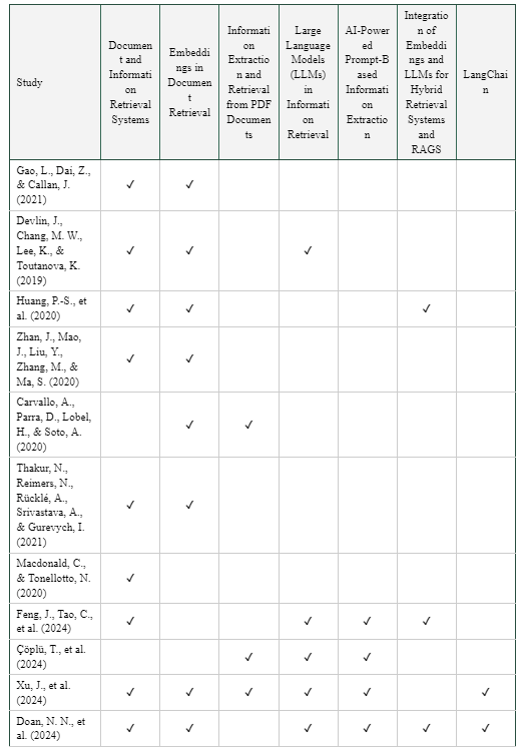
\includegraphics[width=\textwidth]{summary_table.png} % Replace with your image file name
\end{figure}
\begin{figure}[ht]
    \centering
    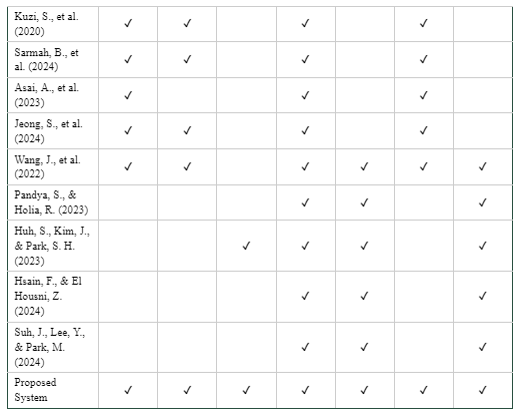
\includegraphics[width=\textwidth]{summary_table1.png} % Replace with your image file name
    \caption{\textit{Summary Features of Related Literatures}}
    \label{fig:related-literature}
\end{figure}


\index{Summary of Related Literatures|)}



% \section[Some Technique Two]{Some Technique Two with Super Long Title Which Will Overrun In Header}
% \index{Some Technique Two|(}
% \blindtext[5]

% Imagine some colourful description on Some Technique Three\index{Some Technique Three}.

% \index{Some Technique Two|)}

